\documentclass{article}
\usepackage{graphicx}
\usepackage{comment}

\begin{document}

\title{Meteor: Real-time Distributed Analytics for a Highly Distributed Environment
}
\author{Umar Javed, Thierry Moreau, Fahad Pervaiz}

\maketitle

\begin{abstract}
We present Meteor, a system optimized for MapReduce tasks on geographically dispersed 
data centers. Traditional solutions for this problem involve all or most of the data backhauled to a central location for processing, making analytics slow and expensive. This is particularly the case for MapReduce-like systems that rely on an all-to-all communication model for aggregation. Meteor avoids this by performing as much of the processing and aggregation at the level of an individual datacenter as possible, thus minimizing communication on expensive inter-datacenter WAN links. Since the aggregation and the resulting reduction on data movement comes at the expense of accuracy of the final result for most analysis tasks, we evaluate the tradeoffs between bandwidth, run-time, and quality of results in Meteor. We implement Meteor as an extension to Apache Spark, an open source in-memory cluster computing stack \cite{1}. 
\end{abstract}

\section{Introduction}

‘Big data’ is getting even bigger due to an explosion in computing devices and the amount of time users spend online. Much of this data is widely distributed due to the global presence of major search and social networking platforms. For example, the data generated and stored by Google’s internal infrastructure, as well as user data collected through its search and advertising services are spread over its multiple datacenters. There are examples of highly physically distributed systems such as sensor and cellular networks where communication links are expensive. On such networks,  backhauling data back to a central server to perform analytics tasks would be slow and impractical. This becomes challenging when much of this data needs to be processed and analyzed in real-time.   

MapReduce is a parallel programming model widely used to analyze large data sets. Traditional MapReduce models assume data stored and jobs scheduled in a single cluster, and is not suitable for an heterogeneous environment where the input data is very large and distributed among multiple clusters. Traditional MapReduce models rely on a centralized master node, through which data has to transit to be scheduled to the worker nodes. Backhauling all the data to a central location quickly becomes slow and expensive over a wide-area network because bandwidth is a scarce resource.

When processing large amounts of physically distributed data, users may prefer a “quick and dirty” result over a correct answer that could take much longer to compute \cite{3, 4}. To this end, we wish to develop a MapReduce infrastructure for data processing on wide-area networks that minimizes communication on expensive links at the expense of result correctness. We explore two ways to reduce data exchange on expensive links between physically distributed nodes: (1) performing the map-reduce jobs locally on each data-center while periodically updating results across data centers, and (2) by reducing the size of the updates sent across data-centers. The first approach could affect convergence and correctness of the results if updates are not frequent enough (see PageRank). The second approach is applicable to a restricted set of queries discussed below (see Top-K).

\section{Case Studies}

We now sketch some examples of data analytics tasks that Meteor provides support for. 

\subsection{Case Study: Top-K}

A top-K query is a common analytic query. For example, a cellular network operator may be interested in finding out the top-K applications users access on their mobile phones. Similarly, a search engine or CDN analyst will be interested in determining the top-K most visited URLs. 
A centralized algorithm for a top-K query will have to transfer all data to a central processing location and then aggregate, requiring a huge amount of bandwidth. For example, consider a network of 1000 cell towers, each connected to 50 mobile devices and generating a record for each device every two seconds. Each record has 200 fields, each field an integer value. The amount of data generated each minute over the network is therefore (1000 x 50 x 30 x 200 x 32) = 10 Gbits. Due to the sheer amount of data needed to be processed, it is much more preferable to process the data locally and do the aggregation only at the end. We plan to provide a top-k operator on top of Spark that implements the multi-round filtering approximate algorithm described in \cite{3}.

\subsection{Case Study: PageRank}

The PageRank algorithm is the cornerstone of Google’s search technology. It is used to rank the many trillions of URLs by importance. PageRank iteratively updates a rank for each webpage by adding up contributions from each page that links to it. On each iteration, the contribution of each page to its neighbors is r/n, where r is its rank, and n is the number of neighbors.
PageRank is an iterative algorithm as opposed to top-K, which is a one-time query. The most bandwidth-hungry stage during a MapReduce implementation of PageRank is the reduce step that aggregates the parent URL for a URL key to compute its rank. We plan to evaluate an approximation where this global reduce step is delayed and done locally instead. 

\subsection{Evaluation}

For our initial evaluation, we will use Emulab \cite{2}. Emulab is suitable since it gives us the ability to configure arbitrary network topologies and link bandwidths. For a start, each node in our Emulab topology will act as a datacenter and a link connecting two nodes will act as a link in the WAN. So far we have configured our environment in Emulab by installing Spark and its dependencies.

Our next steps are:
\begin{itemize}
\item Use Spark for the data analytics examples described above on an emulated distributed topology and show that as the available network bandwidth is reduced, job times increase.
\item Instrument Spark code to measure the bottleneck computations.
\item Implement the operators needed for our examples.
\end{itemize}

For a specific query, we envision our ‘money-graphs’ to be like this:

\begin{figure}[ht]
	\centering
	\begin{minipage}[b]{0.45\linewidth}
		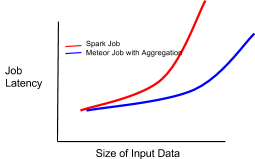
\includegraphics[width=2.3in]{fig_1.png}
		\caption{Latency}
		\label{fig:minipage1}
	\end{minipage}
	\quad
	\begin{minipage}[b]{0.45\linewidth}
		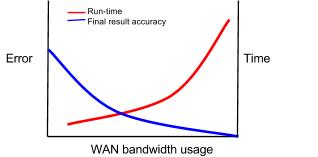
\includegraphics[width=2.6in]{fig_2.png}
		\caption{Error}
		\label{fig:minipage2}
	\end{minipage}
\end{figure}

\begin{comment}
\begin{figure}[ht!]
	\centering
	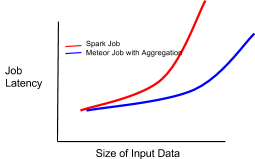
\includegraphics[width=2.4in]{fig_1.png}
	\caption{Latency}
	\label{overflow}
\end{figure}
\begin{figure}[ht!]
	\centering
	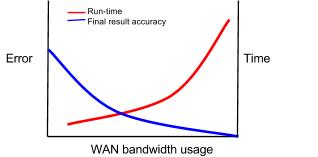
\includegraphics[width=2.6in]{fig_2.png}
	\caption{Error}
	\label{overflow}
\end{figure}
\end{comment}

Here we increase the size of the input data on the x-axis. A Spark job with no topological awareness starts taking longer and longer since the WAN link gets saturated. On the other hand, the corresponding Meteor job takes a lot less time since it uses aggregation to reduce the data needed to be sent over the WAN link. We plan to explore how modulating the bandwidth usage over WAN affects run-time as well as final result accuracy. We expect those result to be highly dependent on the application we are targeting.

\section{Related Work}

Spark, and Spark-streaming \cite{1} are recently developed systems for big-data processing, with Spark-streaming an extension to Spark for streaming applications. The primary innovation of these systems is to keep intermediate data for MapReduce jobs in memory, providing quicker response times. Although these systems provide real-time data analytics with fault tolerance, they assume stable, high bandwidth shared storage, such as HDFS. Meteor, on the other hand, provides fast analytics over multiple datacenters connected by a WAN. We will primarily use Spark as the base for Meteor.  

There’s has been a great deal of theory research on streaming algorithms for distributed queries. These algorithms try to limit message-passing by introducing tolerance for inaccurate final results. For example, distributed top-k monitoring \cite{3} and approximate quantiles \cite{6}. We intend to use many ideas contained in this paper as we figure out the operators that Meteor should support. 

There’s has also been a great deal of research in sensor networks on resource-constrained computing, such as \cite{7}. Although we intend to study and use some of these techniques, our focus is primarily on efficient use of network bandwidth rather than the traditional sensor network focuses such as limited power and/or processing.  

BlinkDB \cite{5} is a massively parallel approximate query engine for running interactive SQL queries on large volumes of data. It allows users to trade-off query accuracy for response time by running queries on data samples. The results are presented to the results to users with meaningful error bars. BlinkDB relies on an optimization framework that maintains multi-dimensional stratified samples from original data over time in order to perform dynamic selection. BlinkDB therefore only applies to centralized databases where dynamic stratification is made possible. It also is restricted to aggregate queries, instead of a broader set of MapReduce jobs.

HOP \cite{4} is an online version of the MapReduce architecture that supports online aggregation, which allows users to see “early returns” from a job as it is being computed. Online aggregation is a technique that provides initial estimates of results several orders of magnitude faster than the final results, by pre-emptively applying the reduce function to the data that a reduce task has received so far at a given point in time. Meteor borrows the idea of  invoking the reduce function on partial map tasks outputs, but applies it in order to reduce the amount of data exchange between workers – not in order to perform interactive analysis.

\begin{thebibliography}{9}

  \bibitem{1} Spark {\em http://spark.incubator.apache.org/}

  \bibitem{2} Emulab {\em http://emulab.net/}

  \bibitem{3} B. Babcock, C. Olston {\em Distributed Top-K Monitoring} In SIGMOD 2003.
  
  \bibitem{4} T. Condie, N. Conway, P. Alvaro, J. M. Hellerstein, K. Elmeleegy, and R. Sears {\em MapReduce Online} In NSDI 2010.
  
  \bibitem{5} S. Agarwal, B. Mozafari, A. Panda, H. Milner, S. Madden, and Ion Stoica {\em BlinkDB: queries with bounded errors and bounded response times on very large data} In EuroSys 2013.
  
  \bibitem{6} C. Cormode, M. Garofalakis, S. Muthukrishnan, R. Rastogi {\em Holistic Aggregates in a Networked World: Distributed Tracking of Approximate Quantiles} In SIGMOD 05.
  
  \bibitem{7} S. Madden, M. J. Franklin, J. M. Hellerstein, and W. Hong {\em TAG: A Tiny AGgregation service for ad-hoc sensor networks} In OSDI, 2002.
  
\end{thebibliography}

\end{document}